\begin{frame}{Featureless Insulators}
\vskip-1.5cm
\begin{columns}[T]
    \begin{column}[T]{.6\textwidth}
        \begin{block}{Definition of `Featureless Insulator'}
            \vskip-1em
            \begin{itemize}
                % 0 T G.S. of quantum Hamiltonians
            \item Gapped 
                %Energy gap to excitations
            \item Symmetric 
                %G.S. Wavefunc preserves all symmetries of the Hamiltonian, no local order parameter - no spontaneous symmetry breaking
            \item No topological order %exotic statistics
                %insulator ->assume that we have a U(1) symmetry by which to define charge
            \item Integer charge per unit cell
                %unit cell -> also assuming discrete translational symmetry
            \item Unique ground state with P.B.C.
                %This can be made into the defining property, all of these others follow from this.
                % Response to change in B.C. can be, with some work, a way to distinguish gapped phases of matter
            \end{itemize}
        \end{block}
    \vskip-0.5cm    
    Examples:
    \end{column}
    \begin{column}[T]{.4\textwidth}
    \begin{figure}[h]
            \centering
            \scalebox{0.7}{
            \input{diagrams/honeycomb3.tex}
            }
            %Atomic insulator
            \caption{\begin{tabular}[t]{l}
                     Bosonic Mott insulator \\
                     with integer filling \end{tabular}}
    \end{figure}
    \end{column}
\end{columns}

\begin{columns}[T]
    \begin{column}[T]{.4\textwidth}
        \vskip-0.5cm
        \begin{figure}[h]
            \centering
            \scalebox{0.6}{
             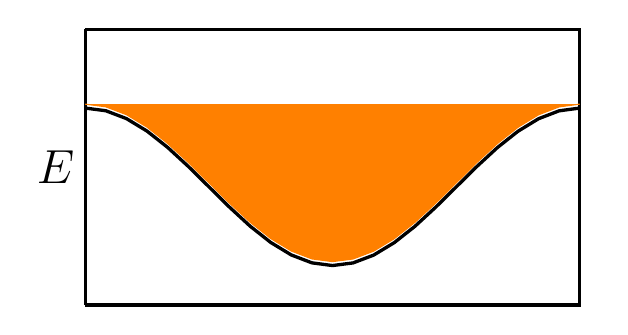
\begin{tikzpicture}[domain=0:6.28]
      \draw[very thick] (0, -2.5) -- (0,1) node[left, midway] {\LARGE $E$} ;
      \draw[very thick] (0, 1)-- (6.28,1) -- (6.28, -2.5) -- (0, -2.5);
      \draw[color=black, very thick] plot (\x,{-1+cos(\x r)}) node[right] {};
      \draw[color=orange, fill] plot (\x,{-0.95+cos(\x r)}) {};
  \end{tikzpicture}
  
            }
        \caption{Band Insulator}
        \end{figure}
    \end{column}
    \begin{column}[T]{.6\textwidth}
        \begin{figure}[h]
            \scalebox{1.4}{
            \input{diagrams/aklt_bare.tex}
            }
            \caption{Heisenberg AF Spin-1 chain}
        \end{figure}
    \end{column}
\end{columns}
\end{frame}